\documentclass[11pt,oneside]{article}
\usepackage[utf8]{inputenc}
\usepackage[a4paper,top=2cm,left=2cm,right=2cm,bottom=2cm]{geometry}
\usepackage{import}
\usepackage[T1]{fontenc}
\usepackage[german,ngerman]{babel}
\usepackage[table]{xcolor}
\usepackage{amsthm, esvect}
\usepackage{mathtools}
\RequirePackage{amssymb, amsfonts, amsmath, latexsym, verbatim, xspace}
\usepackage{systeme}
\usepackage{multicol}
\usepackage{multirow}
\usepackage{framed}
\usepackage{array}
\usepackage{ragged2e}
\usepackage{graphicx}
\usepackage{pdflscape}
\usepackage{epstopdf}
\usepackage{booktabs}
\usepackage{pdfpages}
\usepackage{float} % Allows putting an [H] in \begin{figure} to specify the exact location of the figure
\usepackage{wrapfig} % Allows in-line images such as the example fish picture
\usepackage{tikz, graphicx} % tikz
\usepackage[position=top]{subfig}
\usepackage[bookmarks=true]{hyperref}%Links
\usepackage{enumerate}
\usepackage{enumitem}
\usepackage[german,ruled,vlined,linesnumbered,algosection]{algorithm2e}
\usepackage[labelfont=sf]{caption}
\usepackage{lmodern}
\usepackage{lscape}
\usepackage{tabularx}
\usepackage{systeme}
\usepackage{hhline}
\usepackage{subfiles}
\usepackage{stackengine}
\usepackage{setspace}
\usepackage{MnSymbol}
\usepackage{tcolorbox}
\usepackage{bbm}
\usepackage{url}
\usepackage{xparse}
\usepackage{sectsty}
\usepackage{array}
\usepackage{ragged2e}
\usepackage{listings} %Stellt Code-Snippets sauber dar

% definiert die Sprache
\selectlanguage{German}

% add command for different dates in Swiss fashion
\newcommand{\monthwordlong}[1]{\ifcase#1 \or Januar\or Februar\or März\or April\or Mai\or Juni\or Juli\or August\or September\or Oktober\or November\or Dezember\fi}
\newcommand{\monthwordshort}[1]{\ifcase#1\or Jan\or Feb\or Mar\or Apr\or Mai\or Jun\or Jul\or Aug\or Sept\or Okt\or Nov\or Dez\fi}
\newcommand{\datelong}{\number\day.\:\monthwordlong{\the\month}\:\number\year}
\newcommand{\dateshort}{\number\day.\:\monthwordshort{\the\month}\:\number\year}

% define color of links inside a text
\definecolor{linkblue}{RGB}{0, 0, 80}
\definecolor{plotblue}{RGB}{100, 100, 255}
\definecolor{myblue}{RGB}{8,164,214}
\definecolor{myred}{RGB}{143,42,41}
\definecolor{forestgreen}{RGB}{34,139,34}
\definecolor{highdive}{RGB}{10,169,194}
\definecolor{charcoal}{RGB}{74,74,74}
\hypersetup{
	colorlinks=true,
	linkcolor=linkblue,
	filecolor=magenta,
	urlcolor=plotblue,
	citecolor=linkblue,
	pdfpagemode=FullScreen,
}


\lstdefinestyle{mystyle}{ % definiert den style des Code-Snippets
	%backgroundcolor=\color{backcolour},
	%commentstyle=\color{codegreen},
	%keywordstyle=\color{magenta},
	%numberstyle=\tiny\color{codegray},
	%stringstyle=\color{codepurple},
	basicstyle=\ttfamily\footnotesize,
	breakatwhitespace=false,
	breaklines=true,
	captionpos=b,
	keepspaces=true,
	%numbers=left,
	%numbersep=5pt,
	showspaces=false,
	showstringspaces=false,
	showtabs=false,
	tabsize=4
}
\lstset{style=mystyle}
\usepackage{fancyhdr}

\tcbuselibrary{breakable,skins}
\usetikzlibrary{mindmap,trees}
\newlength\tindent
\setlength{\tindent}{\parindent}
\setlength{\parindent}{0pt}
\renewcommand{\indent}{\hspace*{\tindent}}

\makeatletter
\def\ifEmpty#1{\def\@temp{#1}\ifx\@temp\@empty}
\makeatother

\sectionfont{\underline}
\usetikzlibrary{arrows, petri, topaths, graphs}


% =================== BEISPIEL ====================
\theoremstyle{definition}
\newtheorem{beispiel}{Beispiel}
\renewcommand{\thebeispiel}{\arabic{beispiel}}

% =================== AUFGABE =====================
\newcounter{aufg}[section] % Zähler für die Umgebungen

\newenvironment{aufgabe}[1][]{%
    \refstepcounter{aufg}% Inkrementiere den Zähler
    \begin{tcolorbox}[%
        enhanced,
        overlay unbroken and first={\mytitleaufg[#1]}, % Titelleiste mit Icons wird nicht über Seite gebrochen
        colframe=black,
        boxrule=0pt,
        breakable,
        top=15pt,
        before=\vskip18pt,
    ]
}{%
    \end{tcolorbox}
}

\newcommand{\mytitleaufg}[1][]{% Definiert die Titelleiste und Icons
    \node[fill=black!20,
        rounded corners,
        draw=black,
        text=black,
        line width=1pt,
        inner sep=4pt,
        anchor=west,
        xshift=12pt]
        at (frame.north west){\bfseries Aufgabe \thesection.\theaufg.\ifEmpty{#1}\else\emph{ (#1)}\fi}; % Titel, letzter Teil mit ifempty testet ob #1 leer und macht Klammern und Titel, falls Titelargument übergeben wird bzw. falls #1 leer erscheint nichts - auch keine Klammern

    \node[% Icon
        rounded corners,
        text=black,
        fill=black,
        line width=0pt,
        inner sep=3pt,
        anchor=west,
        xshift=5pt,
        % yshift=-35pt
        ]
        at (frame.north east){
\includegraphics[width=24pt]{../../../Header/Icons/aufgabeicon.png}};
}

% =================== DEFINITION ==================
\newcounter{def}[section] % Zähler für die Umgebungen

\newenvironment{definition}[1][]{%
    \refstepcounter{def}% Inkrementiere den Zähler
    \begin{tcolorbox}[%
        enhanced,
        drop shadow southeast,
        overlay unbroken and first={\mytitledef[#1]}, % Titelleiste mit Icons wird nicht über Seite gebrochen
        colback=blue!5!white,
        colframe=blue!75!black,
        boxrule=2pt,
        breakable,
        top=15pt,
        before=\vskip18pt,
    ]
}{%
    \end{tcolorbox}
}

\newcommand{\mytitledef}[1][]{% Definiert die Titelleiste und Icons
    \node[fill=blue!40!white,
        rounded corners,
        draw=black,
        text=black,
        line width=1pt,
        inner sep=4pt,
        anchor=west,
        xshift=12pt]
        at (frame.north west){\bfseries Definition \thesection.\thedef.\ifEmpty{#1}\else\emph{ (#1)}\fi}; % Titel, letzter Teil mit ifempty testet ob #1 leer und macht Klammern und Titel, falls Titelargument übergeben wird bzw. falls #1 leer erscheint nichts - auch keine Klammern

    \node[% Icon
        rounded corners,
        text=black,
        fill=black,
        line width=0pt,
        inner sep=3pt,
        anchor=west,
        xshift=5pt,
        % yshift=-35pt
        ]
        at (frame.north east){
\includegraphics[width=24pt]{../../../Header/Icons/definitionicon.png}};
}

% =================== NOTATION ====================
\newcounter{nota}[section] % Zähler für die Umgebungen

\newenvironment{notation}[1][]{%
    \refstepcounter{nota}% Inkrementiere den Zähler
    \begin{tcolorbox}[%
        enhanced,
        drop shadow southeast,
        colback=yellow!5!white,
        colframe=yellow!75!black,
        overlay unbroken and first={\mytitlenota[#1]},   % Titelleiste mit Icons wird nicht über Seite gebrochen
        boxrule=2pt,
        breakable,
        top=15pt,
        before=\vskip18pt,
    ]
}{%
    \end{tcolorbox}
}

\newcommand{\mytitlenota}[1][]{% Definiert die Titelleiste und Icons
    \node[fill=yellow!40!white,,
        rounded corners,
        draw=black,
        text=black,
        line width=1pt,
        inner sep=4pt,
        anchor=west,
        xshift=12pt]
        at (frame.north west){\bfseries Notation \thesection.\thenota.\ifEmpty{#1}\else\emph{ (#1)}\fi}; % Titel, letzter Teil mit ifempty testet ob #1 leer und macht Klammern und Titel, falls Titelargument übergeben wird bzw. falls #1 leer erscheint nichts - auch keine Klammern

    \node[% Icon
        rounded corners,
        text=black,
        fill=black,
        line width=0pt,
        inner sep=3pt,
        anchor=west,
        xshift=5pt,
        % yshift=-35pt
        ]
        at (frame.north east){
\includegraphics[width=24pt]{../../../Header/Icons/definitionicon.png}};
}

% =================== SATZ ========================
\newcounter{satz}[section]  % creates a counter and resets it after each chapter

\newenvironment{satz}[1][]{   % Hauptbox mit Satz drin
    \refstepcounter{satz}
    \begin{tcolorbox}[%
        enhanced,
        colback=red!5!white,
        fuzzy halo=2mm with gray,
        colframe=red!75!black,
        overlay unbroken and first={\mytitlesatz[#1]},   % Titelleiste mit Icons wird nicht über Seite gebrochen
        boxrule=2pt,
        breakable,
        top=15pt,
        before=\vskip18pt,
    ]
}{%
    \end{tcolorbox}
}

\newcommand{\mytitlesatz}[1][]{                     % Macht Titelbox und Icons
   \node[fill=red!90!white,
      rounded corners,
      draw=black,,
      text=black,
      line width=1pt,
      inner sep=4pt,
      anchor=west,
      xshift=12pt]
   at (frame.north west){\bfseries Satz \thesection.\thesatz.\ifEmpty{#1}\else\emph{ (#1)}\fi};  % Titel, letzter Teil mit ifx testet ob #1 leer und macht Klammern und Titel, falls Titelargument übergeben wird bzw.  falls #1 leer erscheint nichts - auch keine Klammern

 \node[ % Icon
      rounded corners,
      text=black,
      fill=black,
      line width=0pt,
      inner sep=3pt,
      anchor=west,
      xshift=5pt,
%     yshift=-35pt
]
   at (frame.north east){ 
\includegraphics[width=24pt]{../../../Header/Icons/satzicon.png} };
}

% =================== BEWEIS ======================
\newenvironment{beweis}[1][]{
    \begin{tcolorbox}[
        enhanced,
        overlay unbroken and first={\mybeweis[#1]},     % Titelleiste mit Icons wird nicht über Seite gebrochen
        colback=white,
        colframe=black,
        boxrule=0pt,
        breakable,
        top=15pt,
        before=\vskip18pt,
    ]
}{
        \end{tcolorbox}
}

\newcommand{\mybeweis}[1][]{                     % Macht Titelbox und Icons
   \node[fill=white,
      rounded corners,
      draw=black,
      text=black,
      line width=1pt,
      inner sep=4pt,
      anchor=west,
      xshift=12pt]
   at (frame.north west){\bfseries Beweis \ifEmpty{#1}\else\emph{ (#1)}\fi};  % Titel, letzter Teil mit ifx testet ob #1 leer und macht Klammern und Titel, falls Titelargument übergeben wird bzw.  falls #1 leer erscheint nichts - auch keine Klammern
}

% =================== ALGORITHM ===================
\newcounter{algo}[section]  % creates a counter and resets it after each chapter

\newenvironment{algo}[1][]{   % Hauptbox mit Satz drin
    \refstepcounter{algo}
    \begin{tcolorbox}[%
        enhanced,
        drop shadow southeast,
        colback=yellow!5!white,
        colframe=yellow!75!black,
        overlay unbroken and first={\algotitle[#1]},   % Titelleiste mit Icons wird nicht über Seite gebrochen
        boxrule=2pt,
        breakable,
        top=15pt,
        before=\vskip18pt,
    ]
}{%
    \end{tcolorbox}
}

\newcommand{\algotitle}[1][]{                     % Macht Titelbox und Icons
   \node[fill=yellow!40!white,
      rounded corners,
      draw=black,
      text=black,
      line width=1pt,
      inner sep=4pt,
      anchor=west,
      xshift=12pt]
   at (frame.north west){\bfseries \ifEmpty{#1}{Ablauf}\else{#1}\fi};  % Titel, letzter Teil mit ifx testet ob #1 leer und macht Klammern und Titel, falls Titelargument übergeben wird bzw.  falls #1 leer erscheint nichts - auch keine Klammern

 \node[ % Icon
      rounded corners,
      text=black,
      fill=black,
      line width=0pt,
      inner sep=3pt,
      anchor=west,
      xshift=5pt
      % yshift=-35pt
      ]
   at (frame.north east){ 
\includegraphics[width=24pt]{../../../Header/Icons/algoicon.png} };
}

% ================ Nummerierte Multicol ================
\newenvironment{enumcols}[1][]{
    \begin{enumerate}[label=\alph*)]\begin{multicols}{#1}
}{
    \end{multicols}\end{enumerate}
}



% =================================================
\usetikzlibrary{shapes,arrows}
\tikzstyle{decision} = [diamond, draw, fill=blue!20,
    text width=6em, text badly centered, node distance=4cm, inner sep=0pt]
\tikzstyle{block} = [rectangle, draw, fill=blue!20,
    text width=8em, text centered, rounded corners, minimum height=4em]
\tikzstyle{line} = [draw, -latex']
\tikzstyle{cloud} = [draw, ellipse,fill=red!20, node distance=2cm,
    minimum height=2em]

% Karriertes Papier für Antwort
\newcommand{\karos}[1]{\begin{tikzpicture}\draw[step=0.5cm,color=gray] (0,0) grid (\linewidth,#1 cm);\end{tikzpicture}}
%%
% Header and Footer
%%
\linespread{1.2} % Line spacing
\fancypagestyle{plain}{
	\pagestyle{fancy}
	\lhead{}
	\chead{}
	\rhead{}
	\lfoot{\Autor}
	\cfoot{\Skriptname}
	\rfoot{\thepage}
	\renewcommand{\headrulewidth}{0pt}
	\renewcommand{\footrulewidth}{0.4pt}
}

\pagestyle{fancy}
\fancyhf{}
\rhead{\rightmark}
\lfoot{\leftmark}
\rfoot{\thepage}
\renewcommand{\headrulewidth}{0.2pt}
%\setlength\parindent{0pt} % Uncomment to remove all indentation from paragraphs



%%
% Math Arrows
%%
\newcommand{\same}{\ensuremath{\Longleftrightarrow}}
\renewcommand{\to}{\ensuremath{\longrightarrow}}
\newcommand{\qsame}{\quad\same\quad}
\newcommand{\dsame}{\ensuremath{:\Leftrightarrow}}
\newcommand{\qdsame}{\quad\dsame\quad}
\newcommand{\ldsame}{\ensuremath{:\Longleftrightarrow}}
\newcommand{\samedef}{\ensuremath{\us {\text{def}} \Leftrightarrow}}
\newcommand{\qsamedef}{\quad\samedef\quad}
\newcommand{\lsamedef}{\ensuremath{\us {\text{def}} \Longleftrightarrow}}
\newcommand{\qlsamedef}{\quad\lsamedef\quad}


%%
% Mengendefinitionen
%%
\newcommand{\M}{\ensuremath{\mathcal{M}}}
\newcommand{\N}{\ensuremath{\mathbb{N}}}
\newcommand{\Z}{\ensuremath{\mathbb{Z}}}
\newcommand{\Q}{\ensuremath{\mathbb{Q}}}
\newcommand{\I}{\ensuremath{\mathbb{I}}}
\newcommand{\R}{\ensuremath{\mathbb{R}}}
\newcommand{\C}{\ensuremath{\mathbb{C}}}
\renewcommand{\S}{\ensuremath{\mathbb{S}}}
\newcommand{\Prim}{\ensuremath{\mathbb{P}}}
\newcommand{\0}{\ensuremath{\emptyset}}
\renewcommand{\Re}{\ensuremath{\operatorname{Re}}}
\renewcommand{\Im}{\ensuremath{\operatorname{Im}}}
\newcommand{\strich}{\ensuremath{\big\vert}}

%%
% Mengenoperation
%%
\renewcommand{\nin}{\not\in}


%%
% Logisches Und und Oder
%%
\newcommand{\sand}{\ensuremath{\; \land \;}}
\newcommand{\sor}{\ensuremath{\; \lor \;}}
\renewcommand{\*}{\ensuremath{\cdot}}
\newcommand{\oder}{\vee}
\newcommand{\n}{\neg}
\newcommand{\und}{\wedge}


%%
% Bei Integral, Summe,... die Grenzen über bzw.
% unter das Zeichen
%%
\renewcommand{\d}[1]{\ensuremath{\operatorname{d}\!{#1}}}
\newcommand{\Sum}{\sum\limits}
\newcommand{\Prod}{\prod\limits}
\newcommand{\Min}{\min\limits}
\newcommand{\Max}{\max\limits}
\newcommand{\Lim}{\lim\limits}
\newcommand{\Inf}{\inf\limits}
\newcommand{\Sup}{\sup\limits}
\newcommand{\Liminf}{\liminf\limits}
\newcommand{\Limsup}{\limsup\limits}
%\renewcommand{\Cup}{\bigcup\limits}
%\renewcommand{\Cap}{\bigcap\limits}
\newcommand{\Otimes}{\bigotimes\limits}
\newcommand{\Oplus}{\bigoplus\limits}


%%
% Arcus Cotangens, Logarithmus
%%
\let\oldsin\sin
\renewcommand{\sin}[1]{\oldsin{\left(#1\right)}}
\let\oldcos\cos
\renewcommand{\cos}[1]{\oldcos{\left(#1\right)}}
\let\oldtan\tan
\renewcommand{\tan}[1]{\oldtan{\left(#1\right)}}
\let\oldarcsin\arcsin
\renewcommand{\arcsin}[1]{\oldarcsin{\left(#1\right)}}
\let\oldarccos\arccos
\renewcommand{\arccos}[1]{\oldarccos{\left(#1\right)}}
\let\oldarctan\arctan
\renewcommand{\arctan}[1]{\oldarctan{\left(#1\right)}}
\let\oldln\ln
\renewcommand{\ln}[1]{\oldln{\left(#1\right)}}
\newcommand{\Log}[2]{\ensuremath{\operatorname{log}_{#1}\left(#2\right)}}
\newcommand{\e}{\operatorname{e}}
\renewcommand{\exp}[1]{\ensuremath{\operatorname{\e}^{#1}}}


%%
% Griechische Buchstaben
%%
\renewcommand{\epsilon}{\ensuremath{\varepsilon}}
\renewcommand{\phi}{\varphi}
\renewcommand{\l}{\lambda}
\renewcommand{\t}{\tau}


%%
% Bezeichnungen
%%
\newcommand{\Rgn}{\R_{>0}} % R grösser Null
\newcommand{\Rad}{\operatorname{Rad}}   % Radikal
\newcommand{\kgV}{\operatorname{kgV}}   % Kleinster gemeinsame Vielfache
\newcommand{\ggT}{\operatorname{ggT}}   % Grösster gemeinsame Teiler
\newcommand{\winkel}{\sphericalangle}          % Winkelsymbol
\DeclarePairedDelimiter\abs{\lvert}{\rvert} % besserer Betrag
\makeatletter
\let\oldabs\abs
\def\abs{\@ifstar{\oldabs}{\oldabs*}}
\makeatother


%%
% Vektorgeometrie
%%
\renewcommand{\v}[1]{\vv{#1}}       % besserer Pfeil über Buchstaben
\renewcommand{\vec}[2]{\begingroup\renewcommand{\arraystretch}{1}\left(\begin{array}{c} #1 \\ #2 \end{array}\right)\endgroup}   % two dimensional vector
\renewcommand{\Vec}[3]{\begingroup\renewcommand{\arraystretch}{1}\left(\begin{array}{c} #1 \\ #2 \\ #3 \end{array}\right)\endgroup}      % three dimensional vector


%%
% Text
%%
\newcommand*{\Ueq}[1]{\mathrel{\mathop{=}\limits_{\text{#1}}}}
\newcommand*{\Oeq}[1]{\mathrel{\stackrel{\text{#1}}{=}}}
\newcommand{\utext}[2]{\underbrace{#1}_{\substack{#2}}}
\newcommand{\otext}[2]{$\overbrace{\textrm{#1}}^{\textrm{#2}}$}
\newcommand{\lineortext}[1]{\hspace{0,1cm}\underline{\hspace{0.1cm}\hphantom{#1}\hspace{0.1cm}}\hspace{0,1cm}} % Lückentext erstellen
\newcommand{\gap}[1]{\rule{#1 cm}{1pt}}
\graphicspath{{images/}}

\newcommand{\Skriptname}{Logarithmus}
\newcommand{\Autor}{Jonas Guler (Gu)}

\begin{document}
\begin{titlepage}
	\clearpage
	\title{\Huge\textbf{\Skriptname} \\[1cm]}
	\author{Autor:\\ \Autor}
	\date{\normalsize {Version 1.4}\\ \datelong}
	\maketitle
	\thispagestyle{empty}
	\vfill
	\tableofcontents
\end{titlepage}
\pagenumbering{arabic}
%############################################################################################
\section{Definition des Logarithmus}
	In der Primarschule haben wir die Subtraktion als Umkehrung der Addition kennengelernt. Später haben wir dasselbe mit der Division als Umkehrung der Multiplikation erfahren. Mithilfe der Quadratwurzel waren wir in der Lage, das Quadrieren umzukehren und somit eine Lösung für die Gleichung der Form $x^2=r$ zu finden. In gleichen Sinne wollen wir nun eine Möglichkeit finden, das Potenzieren umdrehen zu können. Das heisst, wir möchten die folgende Gleichung lösen:
	\[2^x=15\]
	\karos{4}
	Die Lösung dieser Gleichung nennt man einen Logarithmus.
	\begin{definition}
		$x=\log{a}{b}$ ist die Lösung der zugehörigen Exponentialgleichung $a^x=b$, wobei $a>0$, $a\neq1$ und $b>0$ gilt.\\
		\emph{Sprich:} Logarithmus zur Basis $a$ von $b$\\
		$\log{a}{b}$ ist also die Zahl, mit der man $a$ potenzieren muss, um $b$ zu erhalten.
	\end{definition}
	\begin{beispiel}\ \\
		\begin{minipage}[t]{0.3\linewidth}
			\begin{enumerate}[label=\alph*)]
				\item Schreibe $6^3=216$ in logarithmischer Form.\\\textit{Lösung:}\[6^3=216 \Leftrightarrow \log{6}{216}=3\]
			\end{enumerate}
		\end{minipage}
		\hfill
		\begin{minipage}[t]{0.3\linewidth}
			\begin{enumerate}[label=\alph*)]
				\setcounter{enumi}{1}
				\item Schreibe $\log{5}{625}=4$ in exponentieller Form.\\\textit{Lösung:}\[\log{5}{625}=4 \Leftrightarrow 5^4=625\]
			\end{enumerate}
		\end{minipage}
		\hfill
		\begin{minipage}[t]{0.3\linewidth}
			\begin{enumerate}[label=\alph*)]
				\setcounter{enumi}{2}
				\item Löse $7^x=230$ auf drei Nachkommastellen.\\\textit{Lösung:}
				\begin{align*}
					7^x=230 \Rightarrow x&=\log{7}{230}\\ &\thickapprox 2.795
				\end{align*}
			\end{enumerate}
		\end{minipage}
	\end{beispiel}
	\begin{aufgabe}
		Schreibe die Exponentialgleichung in logarithmischer Form, die Logarithmusgleichungen in exponentieller Form und löse die Gleichungen auf drei Nachkommastellen genau.
		\begin{enumcols}[3]
				\item $3^4=81$ \item $25^\frac{1}{2}=5$ \item $\left(\frac{1}{6}\right)^{-2}=36$ \item $32^\frac{1}{5}=2$
				\item $\log{3}{9}=2$ \item $\log{6}{216}=3$ \item $\log{5}{0.2}=-1$ \item $\log{0.5}{8}=-3$
				\item $3^x=5$ \item $2^x=10$ \item $4^x=32$ \item $5^x=30$
		\end{enumcols}
	\end{aufgabe}
	\begin{aufgabe}
		\begin{enumerate}
			\item Schreibe den Exponenten $x$ als Logarithmus.
			\begin{enumcols}[4]
				\item $7^x=5$
				\item $p^x=q$
				\item $a^x=\frac{p}{q}$
				\item $\left(\frac{a}{b}\right)^x=c$
				\item $3^{2x}=5$
				\item $4^{x/2}=3$
				\item $\left(\frac{a}{b}\right)^{2x}=c$
				\item $(2\*3)^{3x}=36$
			\end{enumcols}
			\item Notiere die Gleichung als Exponentialgleichung.
			\begin{enumcols}[4]
				\item $x=\log{u}{v}$
				\item $x=\log{2}{12}$
				\item $y=\log{\sqrt{2}}{x}$
				\item $z=\log{c}{\frac{2}{d}}$
			\end{enumcols}
		\end{enumerate}
	\end{aufgabe}
	Wir sind nun also in der Lage, auch schwierigere Exponentialgleichungen zu lösen.
	\begin{aufgabe}
		Löse die folgenden Exponentialgleichungen und überprüfe deine Lösung mit dem Taschenrechner.
		\begin{enumcols}[2]
				\item $10^{2x-3}=4$ \item $2^{x^2-1}=100$ \item $3^{4x-2}+100=0$ \item $\frac{1}{2}\*4^{x-2}=6$
				\item $7^{4-x}=1000$ \item $4^{2x-5}=3$
		\end{enumcols}
	\end{aufgabe}
	\newpage


\section{Rechenregeln}
	Wir haben nun in den Aufgaben einige Umformungen verwendet, die direkt aus der Definition folgen. Da diese für die Beweise der Rechenregeln mit Logarithmen entscheidend sind, sind sie hier nochmals allgemein zusammengefasst.
	\begin{satz}
		Auch hier gilt $a>0$, $a\neq0$ und $b>0$. $r$ sei eine beliebige Zahl ($r\in\R$).
		\begin{enumerate}
			\item $a^{\log{a}{b}}=b$
			\item $\log{a}{a^r}=r$
			\item $\log{a}{1}=0$
		\end{enumerate}
	\end{satz}
	Wir möchten nun die weiteren Rechenregeln anhand einer Beispielaufgabe entdecken.
	\begin{aufgabe}
		Durch systematisches Probieren möchten wir die Regeln selbst entdecken. Betrachte dazu die Tabelle rechts.
		\begingroup
		\renewcommand{\arraystretch}{1.5}
		\begin{table}[H]
			\centering
			\begin{tabular}{c|c|c|c|c|c|c|c}
				$x$ & $2$ & $4$ & $8$ & $16$ & $32$ & $64$ & $128$ \\\hline
				$\log{2}{x}$ & $1$ & $2$ & $3$ & $4$ & $5$ & $6$ & $7$
			\end{tabular}
		\end{table}
		\endgroup
		\begin{enumerate}[label=\alph*)]
			\item Wie hängt der Wert des Terms $\log{2}{u\*v}$ von $\log{2}{u}$ und $\log{2}{v}$ ab? Vergleiche dazu die folgenden Terme.\\
			$\log{2}{2\*4}$ mit $\log{2}{2}$ und $\log{2}{4}$\vspace{5pt}\\\karos{1.5}
			$\log{2}{2\*8}$ mit $\log{2}{2}$ und $\log{2}{8}$\vspace{5pt}\\\karos{1.5}
			$\log{2}{4\*8}$ mit $\log{2}{4}$ und $\log{2}{8}$\vspace{5pt}\\\karos{1.5}
			$\log{2}{8\*16}$ mit $\log{2}{8}$ und $\log{2}{16}$\vspace{5pt}\\\karos{1.5}
			Stelle eine Vermutung für eine Rechenregel auf und überprüfe sie an eigenen Beispielen.
			\[\log{a}{u\*v}=\gap{5}\]
			\item Verfahre genauso wie in Teilaufgabe a) mit $\log{2}{\frac{u}{v}}$.\\
			$\log{2}{\frac{32}{4}}$ mit $\log{2}{32}$ und $\log{2}{4}$\vspace{5pt}\\\karos{1.5}
			$\log{2}{\frac{64}{32}}$ mit $\log{2}{64}$ und $\log{2}{32}$\vspace{5pt}\\\karos{1.5}
			$\log{2}{\frac{128}{16}}$ mit $\log{2}{128}$ und $\log{2}{16}$\vspace{5pt}\\\karos{1.5}
			$\log{2}{\frac{8}{64}}$ mit $\log{2}{8}$ und $\log{2}{64}$\vspace{5pt}\\\karos{1.5}
			Stelle eine Vermutung für eine Rechenregel auf und überprüfe sie an eigenen Beispielen.
			\[\log{a}{\frac{u}{v}}=\gap{5}\]
		\end{enumerate}
	\end{aufgabe}
	Wir können also die Regeln allgemein zusammenfassen und noch mit einer weiteren Regel, der Potenzregel, erweitern.
	\begin{satz}
		\label{satz:logarithmusgesetze}
		Seien $a>0$, $a\neq0$ sowie $u>0$ und $v>0$. $r$ ist wiederum eine beliebige Zahl ($r\in\R$).
		\begin{enumerate}[label=\Roman*.]
			\item Produktregel: \[\gap{7}\]
			\item Quotientenregel: \[\gap{7}\]
			\item Potenzregel: \[\log{a}{u^r}=r\*\log{a}{u}\]
		\end{enumerate}
	\end{satz}
	\begin{aufgabe}
		Vereinfache die folgenden Terme so weit wie möglich.
		\begin{enumcols}[4]
				\item $\log{12}{144}$
				\item $\log{10}{0.001}$
				\item $\log{a}{\frac{1}{a^2}}$
				\item $5^{\log{5}{10}}$
				\item $\log{5}{25\sqrt{5}}$
				\item $\log{x}{x\sqrt{x}}$
				\item $\log{a}{\frac{1}{\sqrt{a}}}$
				\item $\log{m}{\sqrt{m^5}}$
		\end{enumcols}
	\end{aufgabe}
	\begin{aufgabe}
		\begin{enumerate}
			\item Fasse die folgenden Terme zu einem einzigen Logarithmus zusammen und vereinfache so weit wie möglich.
			\begin{enumcols}[2]
				\item $\log{a}{2}+\log{a}{7}-\log{a}{14}$
				\item $\frac{1}{3}\*\log{a}{8}-\log{a}{2}$
				\item $3\*\log{a}{25}-2\*\log{a}{125}$
				\item $\log{a}{3}-2\*\log{a}{5}+\frac{1}{2}\*\log{a}{4}$
				\item $\log{a}{m^2}-\log{a}{m}$
				\item $\log{a}{x^3}-3\*\log{a}{\frac{1}{x}}$
				\item $\log{a}{\frac{1}{y^3}}-\log{a}{\frac{1}{y^4}}$
				\item $\ds\frac{\log{a}{x^5}}{\log{a}{x^4}}$
				\item $\log{a}{b}+\log{a}{c}-\log{a}{d}\log{a}{e}$
				\item $3\*\log{a}{b}+2\*\log{a}{c}-4\*\log{a}{d}$
				\item $-\log{a}{x}-\log{a}{y}-\log{a}{z}$
				\item $\frac{1}{4}\*\log{a}{x^3}-\frac{1}{2}\*\log{a}{y}+3\*\log{a}{z}$
				\item $2\*\log{a}{x}-5\*\left(\log{a}{u}+\log{a}{v}\right)$
				\item $\log{a}{x^{\frac{1}{4}}}+\log{a}{x^{\frac{3}{2}}}-\log{a}{\sqrt{x}}$
			\end{enumcols}
			\item Ist die folgende Umformung richtig oder falsch? Begründe deine Antwort.
			\begin{enumcols}[2]
				\item $\log{a}{u+2}=\log{a}{u}+\log{a}{2}$
				\item $\log{a}{u+u}=\log{a}{2}+\log{a}{u}$
				\item $\log{a}{3\*v}=3\*\log{a}{v}$
				\item $\log{a}{u-4}=\frac{\log{a}{u}}{\log{a}{4}}$
				\item $\log{a}{\frac{2}{3}}=\frac{\log{a}{2}}{\log{a}{3}}$
				\item $\log{a}{3\*u}=3\*\log{a}{u}$
			\end{enumcols}
		\end{enumerate}
	\end{aufgabe}
	\begin{aufgabe}
		Forme die ausgeschriebenen Ausdrücke soweit um, bis nur noch ein Logarithmus übrig bleibt oder umgekehrt. \\\footnotesize\textit{Tipp: Falls kein Logarithmusgesetz anwendbar scheint, versuche den Ausdruck in ein Produkt umzuwandeln.}\normalsize
		\begin{enumcols}[2]
				\item $2\*\log{3}{x}-\log{3}{5}$
				\item $3\*\log{2}{x}-4\*\log{2}{x+3}+\log{2}{y}$
				\item $\log{2}{x^2-25}-2\*\log{2}{x-5}$
				\item $2+\frac{\log{10}{x}}{3}-\log{10}{x}$
				\item $\log{a}{b^2-b}$
				\item $\log{a}{\frac{x^2y}{u-v}}$
				\item $\log{a}{\sqrt{\frac{x}{y}}\*c^5}$
				\item $\log{a}{\frac{12xy^5}{5uv^3}}$
		\end{enumcols}
	\end{aufgabe}
	\begin{aufgabe}[für die Schnellen]
		Beweise die Potenzregel aus Satz \ref{satz:logarithmusgesetze}.
	\end{aufgabe}



\newpage
\section{Logarithmen zu Zeiten von Jost Bürgi $(1552-1632)$}


\newpage
\section{Die Logarithmusfunktion}
	Der Logarithmus beschreibt also die exakte Lösung einer Exponentialgleichung. Das heisst, wenn wir mit der natürlichen Exponentialfunktion $f(x)=\exp{x}$ starten, dann ordnet der natürliche Logarithmus jedem Bild $f(x)$ sein Argument $x$ zu. Der Logarithmus dreht also diese Funktion um.
	\begin{aufgabe}
		Betrachten wir die drei Einführungsbeispiele der Exponentialfunktion (Wasserpflanze, Taschengeld (Angebot B), Uran-Atome). Zeichne für alle drei Funktionen den Funktionsgraph, wenn du das Bild mit dem Argument vertauschst.\vspace{2pt}\newline
		\begin{tikzpicture}[cross/.style={draw, cross out, minimum size=2*(#1-1pt), inner sep=0pt, outer sep=0pt}, x=20mm, y=10mm,
			>=latex,   %Voreinstellung für Pfeilspitzen
			font=\footnotesize, scale=1]
			%Raster zeichnen
			\draw [color=gray!50]  [step=5mm] (-0,-0) grid (5.3,5.3);
			% Achsen zeichnen
			\draw[->,thick] (-0.3,0) -- (5.5,0) node[right=20pt, below] {\normalsize $x$ in m$^2$};
			\draw[->,thick] (0,-0.3) -- (0,5.5) node[above, left] {\normalsize $y$ in Monaten};
			% Achsen beschriften
			\foreach \x/\label in {1/10'000,2/20'000,3/30'000,4/40'000,5/50'000} \draw (\x,-.1) -- (\x,.1) node[below=5pt] {$\label$};
			\foreach \y in {1,2,...,5} \draw (-.05,\y) -- (.05,\y) node[left=5pt] {$\y$};
			% Besserer Ursprung
			\draw[color=black] (0pt,-7pt) node[right] {$0$};
			%Funktionen zeichnen:
			\clip(-0.3,-0.3) rectangle (5.3,5.3); %Bildbereich
			%Beschriftung
			%\node[blue]  at (11,5) {\normalsize$f$};
		\end{tikzpicture}

		\begin{tikzpicture}[cross/.style={draw, cross out, minimum size=2*(#1-1pt), inner sep=0pt, outer sep=0pt}, x=0.5mm, y=10mm,
			>=latex,   %Voreinstellung für Pfeilspitzen
			font=\footnotesize, scale=0.9]
			%Raster zeichnen
			\draw [color=gray!50]  [step=5mm] (-0,-0) grid (204,12.1);
			% Achsen zeichnen
			\draw[->,thick] (-5,0) -- (210,0) node[right=25pt, below] {\normalsize $x$ in CHF};
			\draw[->,thick] (0,-0.3) -- (0,12.5) node[above, left] {\normalsize $y$ in Tage};
			% Achsen beschriften
			\foreach \x in {20,40,...,200} \draw (\x,-.1) -- (\x,.1) node[below=4pt] {$\x$};
			\foreach \y in {1,2,...,12} \draw (-2.,\y) -- (2.,\y) node[left=4pt] {$\y$};
			% Besserer Ursprung
			\draw[color=black] (0pt,-7pt) node[right] {$0$};
			%Funktionen zeichnen:
			%\clip(-0.3,-0.3) rectangle (60.8,6.8); %Bildbereich
			%Beschriftung
			%\node[blue]  at (11,5) {\normalsize$f$};
		\end{tikzpicture}

		\begin{tikzpicture}[cross/.style={draw, cross out, minimum size=2*(#1-1pt), inner sep=0pt, outer sep=0pt}, x=2.4mm, y=14.4mm,
			>=latex,   %Voreinstellung für Pfeilspitzen
			font=\footnotesize, scale=1]
			%Raster zeichnen
			\draw [color=gray!50]  [step=4.8mm] (-0,-0) grid (32.4,4.1);
			% Achsen zeichnen
			\draw[->,thick] (-1,0) -- (33,0) node[below=8pt, right] {\normalsize $x$};
			\draw[->,thick] (0,-0.3) -- (0,4.5) node[above, left] {\normalsize $y$ in h};
			% Achsen beschriften
			\foreach \x/\label in {5/5'000,10/10'000,15/15'000,20/20'000,25/25'000,30/30'000} \draw (\x,-.05) -- (\x,.05) node[below=4pt] {$\label$};
			\foreach \y in {1,2,...,12} \draw (-.2,\y/3) -- (.2,\y/3) node[left=4pt] {$\frac{\y}{3}$};
			% Besserer Ursprung
			\draw[color=black] (0pt,-7pt) node[right] {$0$};
			%Funktionen zeichnen:
			%\clip(-0.3,-0.3) rectangle (60.8,6.8); %Bildbereich
			%Beschriftung
			%\node[blue]  at (11,5) {\normalsize$f$};
		\end{tikzpicture}
	\end{aufgabe}
	In den drei Beispielen sehen wir eine neue Klasse von Funktionen. Diese Graphen haben alle eine Funktionsgleichung der Form: \[f(x)=\log{a}{\frac{x}{b}}\] mit $b\in\R$ und $a\in\R^+\backslash\left\{1\right\}$. Für die weitere Diskussion der Eigenschaften fixieren wir $b=1$.
	\begin{definition}
		Eine Logarithmusfunktion ist eine Funktion der Form \[f(x)=\log{a}{x}\]
		mit $a\in\R^+\backslash\left\{1\right\}$.
	\end{definition}
	\begin{beispiel}
		Betrachten wir die beiden folgenden Beispiele: \[\textcolor{blue}{f}(x)=\log{2}{x} \text{ und } \textcolor{forestgreen}{g}(x)=\log{\frac{1}{2}}{x}.\]
		\begin{minipage}{0.48\linewidth}
			\centering
			\begin{tikzpicture}[cross/.style={draw, cross out, minimum size=2*(#1-1pt), inner sep=0pt, outer sep=0pt}, x=4mm, y=10mm,
				>=latex,   %Voreinstellung für Pfeilspitzen
				font=\footnotesize, scale=0.8]
				%Raster zeichnen
				%\draw [color=gray!50]  [step=8mm] (-0,-0) grid (32.4,4.1);
				% Achsen zeichnen
				\draw[->,thick] (-1,0) -- (16,0) node[left, below] {\normalsize $x$};
				\draw[->,thick] (0,-3.3) -- (0,4.5) node[above, left=4pt] {\normalsize $y$};
				% Achsen beschriften
				\foreach \x in {2,4,...,14} \draw (\x,-.1) -- (\x,.1) node[below=4pt] {$\x$};
				\foreach \y in {-3,-2,-1,1,2,...,4} \draw (-.3,\y) -- (.3,\y) node[left=4pt] {$\y$};
				% Besserer Ursprung
				\draw[color=black] (0pt,-7pt) node[left] {$0$};
				%Funktionen zeichnen:
				\clip(-3,-3.3) rectangle (14.2,4.1); %Bildbereich
				\draw[blue,domain=0.1:14,samples=100] plot (\x, {ln(\x)/ln(2)}) node[below] {$f$};
				%Beschriftung
				%\node[blue]  at (11,5) {\normalsize$f$};
			\end{tikzpicture}
		\end{minipage}
		\hfill
		\begin{minipage}{0.48\linewidth}
			\centering
			\begin{tikzpicture}[cross/.style={draw, cross out, minimum size=2*(#1-1pt), inner sep=0pt, outer sep=0pt}, x=4mm, y=10mm,
				>=latex,   %Voreinstellung für Pfeilspitzen
				font=\footnotesize, scale=0.8]
				%Raster zeichnen
				%\draw [color=gray!50]  [step=8mm] (-0,-0) grid (32.4,4.1);
				% Achsen zeichnen
				\draw[->,thick] (-1,0) -- (16,0) node[left, below] {\normalsize $x$};
				\draw[->,thick] (0,-3.3) -- (0,4.5) node[above, left=4pt] {\normalsize $y$};
				% Achsen beschriften
				\foreach \x in {2,4,...,14} \draw (\x,-.1) -- (\x,.1) node[below=4pt] {$\x$};
				\foreach \y in {-3,-2,-1,1,2,...,4} \draw (-.3,\y) -- (.3,\y) node[left=4pt] {$\y$};
				% Besserer Ursprung
				\draw[color=black] (0pt,-7pt) node[left] {$0$};
				%Funktionen zeichnen:
				\clip(-3,-3.3) rectangle (14.2,4.1); %Bildbereich
				\draw[forestgreen,domain=0.1:10,samples=100] plot (\x, {ln(\x)/ln(0.5)}) node[above] {$g$};
				%Beschriftung
				%\node[blue]  at (11,5) {\normalsize$f$};
			\end{tikzpicture}
		\end{minipage}
	\end{beispiel}
	\begin{satz}[Wachstumsverhalten]
		Eine Funktion der Form $h(x)=\log{a}{x}$ zeigt folgendes Wachstumsverhalten in Abhängigkeit der Basis $a$:
		\begin{itemize}
			\item \rule{10cm}{1pt}
			\item \rule{10cm}{1pt}
		\end{itemize}
	\end{satz}
	Die beiden Funktionen im Beispiel besitzen aber auch sehr viele Gemeinsamkeiten. Bei beiden ist der Einfluss des Parameters $a$ entscheidend für die Gestalt der Kurve. Der Definitions- und Wertebereich ist ebenfalls bei beiden Funktionen gleich. Fasse im folgenden Satz deine Beobachtungen zusammen.
	\begin{satz}[Eigenschaften]
		Die Funktion $f(x)=\log{a}{x}$ hat folgende Eigenschaften:
		\begin{itemize}
			\item Der Definitionsbereich ist \gap{2} und der Wertebereich ist \gap{2}.
			\item Die Funktion hat eine einzige Nullstelle bei \gap{2}.
			\item Monotonie:\begin{itemize}
				\item Für $a>1$ ist die Funktion streng monoton wachsend.
				\item Für $0<a<1$ ist die Funktion streng monoton fallend.\end{itemize}
			\item Asymptotisches Verhalten:\begin{itemize}
				\item Die $y-$Achse ist eine Asymptote.\end{itemize}
		\end{itemize}
	\end{satz}
	\begin{aufgabe}
		\begin{enumerate}
			\item Zeichne die Logarithmusfunktionen von $f:y=\log{a}{x}$ für $a=2,3,\frac{1}{2},\frac{1}{4}$ im gleichen Koordinatensystem unten.
			\begin{figure}[H]
				\centering
				\begin{tikzpicture}[cross/.style={draw, cross out, minimum size=2*(#1-1pt), inner sep=0pt, outer sep=0pt}, x=10mm, y=10mm,
					>=latex,   %Voreinstellung für Pfeilspitzen
					font=\footnotesize, scale=0.9]
					\begin{scope}[on background layer]
						\fill[white] (-1,-4.5) rectangle (9,5);
					\end{scope}
					%Raster zeichnen
					\draw [color=gray!50]  [step=10mm] (-0.2,-4.2) grid (8.2,4.2);
					% Achsen zeichnen
					\draw[->,thick] (-0.7,0) -- (8.7,0) node[left, below] {\normalsize $x$};
					\draw[->,thick] (0,-4.3) -- (0,4.5) node[above, left=4pt] {\normalsize $y$};
					% Achsen beschriften
					\foreach \x in {1,2,...,8} \draw (\x,-.1) -- (\x,.1) node[below=4pt] {$\x$};
					\foreach \y in {-4,...,-2,-1,1,2,...,4} \draw (-.1,\y) -- (.1,\y) node[left=4pt] {$\y$};
					% Besserer Ursprung
					\draw[color=black] (0pt,-7pt) node[left] {$0$};
					%Funktionen zeichnen:
					\clip(0,-4.2) rectangle (8.2,4.2); %Bildbereich
					%Beschriftung
					%\node[blue]  at (11,5) {\normalsize$f$};
				\end{tikzpicture}
			\end{figure}
			\item Der Punkt $P$ liegt auf der Funktion der Form $f:y=\log{a}{x}$. Berechne $a$.
			\begin{enumcols}[4]
				\item $P\left(9\:\vert\:2\right)$
				\item $P\left(4\:\vert\:\frac{1}{2}\right)$
				\item $P\left(\frac{1}{8}\:\vert\:-\frac{3}{4}\right)$
				\item $P\left(2\:\vert\:-5\right)$
			\end{enumcols}
			\item Gib die Funktionsgleichung der Umkehrfunktion an.
			\begin{enumcols}[4]
				\item $f:y=10^x$
				\item $f:y=\left(\frac{1}{3}\right)^x$
				\item $f:y=2^{3x}$
				\item $f:y=\log{5}{\sqrt{x}}$
			\end{enumcols}
			\item Jede Wertetabelle gehört zu einer Logarithmusfunktion der Form $f:y=\log{a}{x}+c$. Wie lautet die Funktionsgleichung?\vspace*{7pt}\newline
			\begin{minipage}{0.3\linewidth}
				\begin{tabular}{c|c|c|c|c}
					$x$ & $1$ & $3$ & $9$ & $243$ \\\hline
					$f(x)$ & $0$ & $1$ & $2$ & $5$ \\
				\end{tabular}
			\end{minipage}
			\hfill
			\begin{minipage}{0.3\linewidth}
				\begin{tabular}{c|c|c|c|c}
					$x$ & $\frac{1}{8}$ & $2$ & $16$ & $32$ \\\hline
					$f(x)$ & $3$ & $-1$ & $-4$ & $-5$ \\
				\end{tabular}
			\end{minipage}
			\hfill
			\begin{minipage}{0.3\linewidth}
				\begin{tabular}{c|c|c|c|c}
					$x$ & $2$ & $12$ & $72$ & $432$ \\\hline
					$f(x)$ & $1$ & $2$ & $3$ & $4$ \\
				\end{tabular}
			\end{minipage}
		\end{enumerate}
	\end{aufgabe}
	\begin{aufgabe}
			\begin{minipage}{0.57\linewidth}
				Ordne zuerst die Funktionsgleichungen den Graphen zu.
				\begin{align*}
					f(x)&=\log{2}{x}\\
					g(x)&=\log{2}{x-1}\\
					h(x)&=\log{2}{x}-1
				\end{align*}
			\end{minipage}
			\hfill
			\begin{minipage}{0.4\linewidth}
				\centering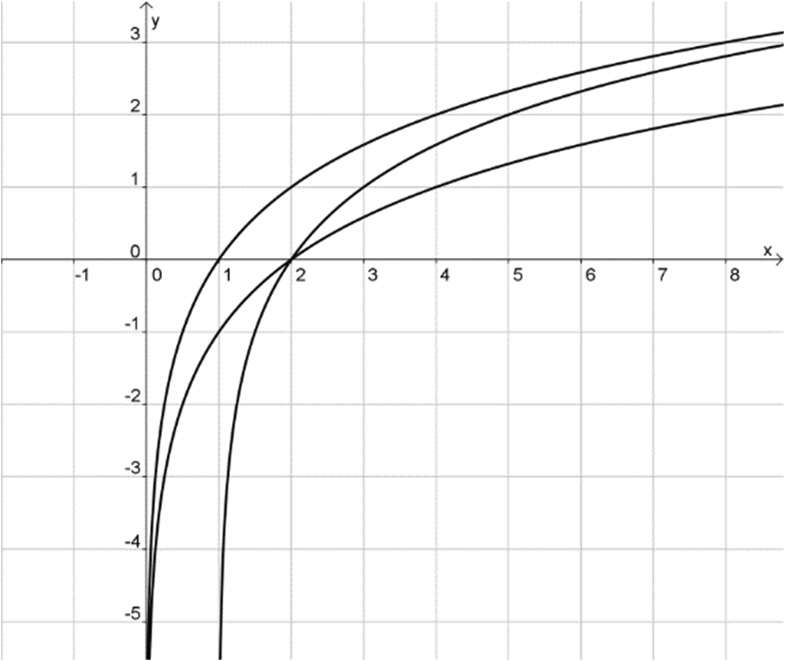
\includegraphics[scale=0.18]{images/shiftedLog1.png}
			\end{minipage}\vspace{22pt}
			Beschreibe danach den Einfluss der beiden verschiedenen Parameter $b$ und $c$ der allgemeinen Funktion \[f(x)=\log{a}{x-b}+c.\] Vergleiche dazu das \href{https://www.geogebra.org/m/qungkacj}{Geogebra-Applet}\footnotemark.
	\end{aufgabe}
	\begin{aufgabe}
		Gib die Gleichung der Logarithmusfunktion an. Die gestrichelten Geraden sind Asymptoten.
		\begin{figure}[H]
			\centering
			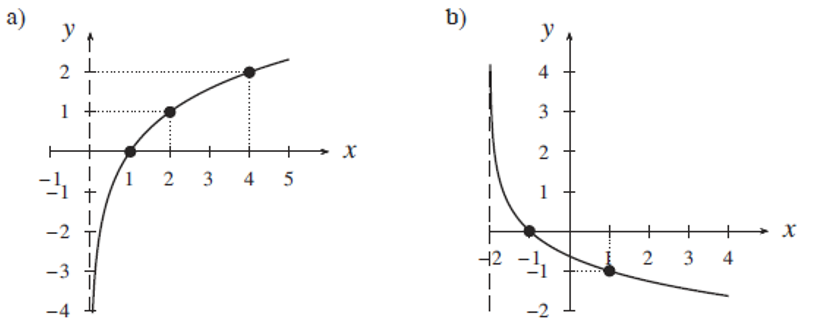
\includegraphics[scale=0.6]{aufgloggraph.png}
		\end{figure}
	\end{aufgabe}
	\footnotetext{\url{https://www.geogebra.org/m/qungkacj}}


\newpage
\section{Verschiedene Anwendungen}
\subsection{Lautstärke}
	\begin{figure}[ht]
		\centering
		\textbf{Empfinden wir zwei schreiende Kinder doppelt so laut wie eines?}
		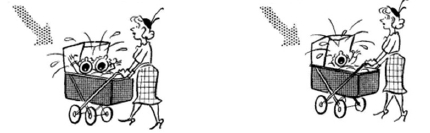
\includegraphics[scale=0.9]{Schreihals.png}
	\end{figure}
	\begin{wrapfigure}{r}{0.3\textwidth}
		\center{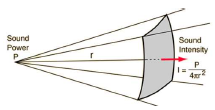
\includegraphics[scale=0.8]{SoundIntensity.png}}
	\end{wrapfigure}
	Wie ihr vielleicht wisst, breitet sich der Schall mittels Kompression und Dekompression der Luft aus. Das heisst, wir einen Ton hören, wenn in der Luft gewisse Energie vorhanden ist, die Schallwellen erzeugen. Je weiter weg wir vom Ursprung der Schallquelle sind, desto leiser nehmen wir den Ton wahr. Nehmen wir die Frage zu Beginn nochmals auf: Empfinden wir zwei schreiende Kinder als doppelt so laut wie eines? Intuitiv würde ich diese Frage mit \flqq Nein\frqq\:beantworten. Dies kann auch genau erklärt werden, denn unser Gehör funktioniert mit einer logarithmischen Skala. Aus diesem Grund wird die Schallenergie eines Geräusches mit dem leisest hörbaren verglichen. Daraus lässt sich die Lautstärke wie folgt definieren:

	\begin{definition}
		\[\text{Lautstärke [in dB (Dezibel)]}=10\*\log{10}{\frac{\textcolor{red}{I}}{I_0}},\]
		wobei $I_0=\left(10^{-12}\frac{W}{m^2}\right)$ die Hörschwelle und $\textcolor{red}{I}$ die gemessene Schallenergie sind.
	\end{definition}
	In der Graphik unten sind einerseits einige Lautstärken abgebildet. $0$dB ist das leiseste, was ein menschliches Gehör feststellen kann und interessanterweise ist die Schmerzgrenze bei $130$dB. Lärm der lauter ist als die Schmerzgrenze kann zu abruptem Hörverlust führen. Betrachten wir den Graphen auf der Mitte, so sehen wir die Ähnlichkeit zur klassischen Logarithmusfunktion. Vergleicht man die Werte, so führt eine Verdoppelung der Schallenergie zu einem Anstieg um lediglich $3$ Dezibel.\newline
	\begin{minipage}{0.3\linewidth}
		\centering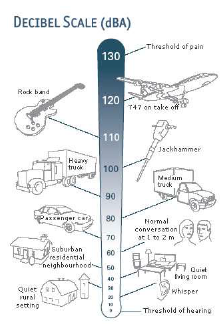
\includegraphics[scale=0.4]{DezibelSkala.png}
	\end{minipage}
	\hfill
	\begin{minipage}{0.3\linewidth}
		\centering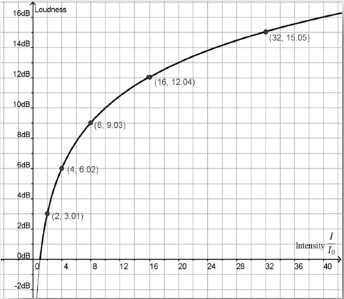
\includegraphics[scale=0.4]{DezibelGraph.png}
	\end{minipage}
	\hfill
	\begin{minipage}{0.3\linewidth}
		\centering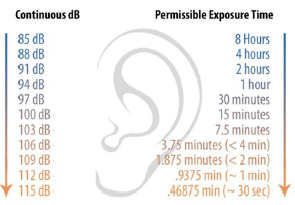
\includegraphics[scale=0.6]{ExposureTime.png}
	\end{minipage}\newline
	Falls das Gehör zu lange grossem Lärm ausgesetzt ist, kann dies zu Gehörverlust führen. Wird die Schallenergie verdoppelt, also $+3$dB, so halbiert sich die Belastungszeit für diese Lautstärke. Eine Aufstellung für die Belastungszeiten kann in der Abbildung auf der rechten Seite abgelesen werden.
	\begin{aufgabe}
		Wähle aus den folgenden Anwendungen eine aus, die dich interessiert.
		\begin{enumcols}[3]
			\item Richterskala \item ph-Werte \item C-14 Methode
		\end{enumcols}
		Beschreibe deine Anwendung in maximal einer A4-Seite. Beantworte dabei folgende Leitfragen:
		\begin{enumerate}
			\item In welchem Zusammenhang wird sie verwendet? Wozu wird sie verwendet?
			\item Wie ist die Anwendung definiert? (Mache dabei den Bezug zum Logarithmus sichtbar.)
			\item Erkläre warum die Verwendung von Logarithmus sinnvoll ist.
			\item Suche ein Beispiel, welches die Anwendung zeigt.
			\item Ergänze allfällige \flqq Fun Facts\frqq.
		\end{enumerate}
	\end{aufgabe}
	\newpage



\subsection*{History}
\begin{table}[H]
	\centering
	\begin{tabular}{|p{13mm}|p{20mm}|p{30mm}|p{70mm}|}\hline
		%\multicolumn{4}{|l|}{History}\\\hline
		Version & Datum & Person & Bemerkung \\\hline
		$1.1$ & 22.12.2023 & Jonas Guler & Kapitel erstellt \\\hline
		$1.2$ & 12.10.2024 & Jonas Guler & Anwendungen ergänzen \\\hline
		$1.3$ & 21.10.2025 & Jonas Guler & Korrekturen einpflegen und Aufgaben ergänzen \\\hline
		$1.4$ & 31.07.2026 & Jonas Guler & Abschnitt zum Basiswechselsatz in Anhang verschoben, da im Lehrplan nicht vorgesehen und mit neuen TR nicht länger motiviert werden kann. \\\hline
	\end{tabular}
\end{table}
\newpage

\appendix
\begingroup % group removes the section entries to be displayed in toc
\let\oldaddcontentsline\addcontentsline
\renewcommand{\addcontentsline}[3]{}
\section{Der Basiswechselsatz}
	\begin{definition}
		Wir definieren drei spezielle Logarithmen.
		\begin{table}[H]
			\centering
			\begin{tabular}{l c}
				Logarithmus zur Basis $10$: & $\log{10}{x}=\operatorname{log}(x)$\\
				Logarithmus zur Basis $2$: & $\log{2}{x}=\operatorname{lb}(x)$\\
				Logarithmus zur Basis $\e$: & $\log{\e}{x}=\ln{x}$
			\end{tabular}
		\end{table}
	\end{definition}
	\begin{minipage}{0.6\linewidth}
	Wir haben verschiedene Methoden kennengelernt, wie wir Logarithmen vereinfachen können. Können wir aber diese Logarithmen auch mit einfachen Mittel, wie beispielsweise unserem Handy Taschenrechner, approximieren?
	\end{minipage}
	\hfill
	\begin{minipage}{0.35\linewidth}
	\centering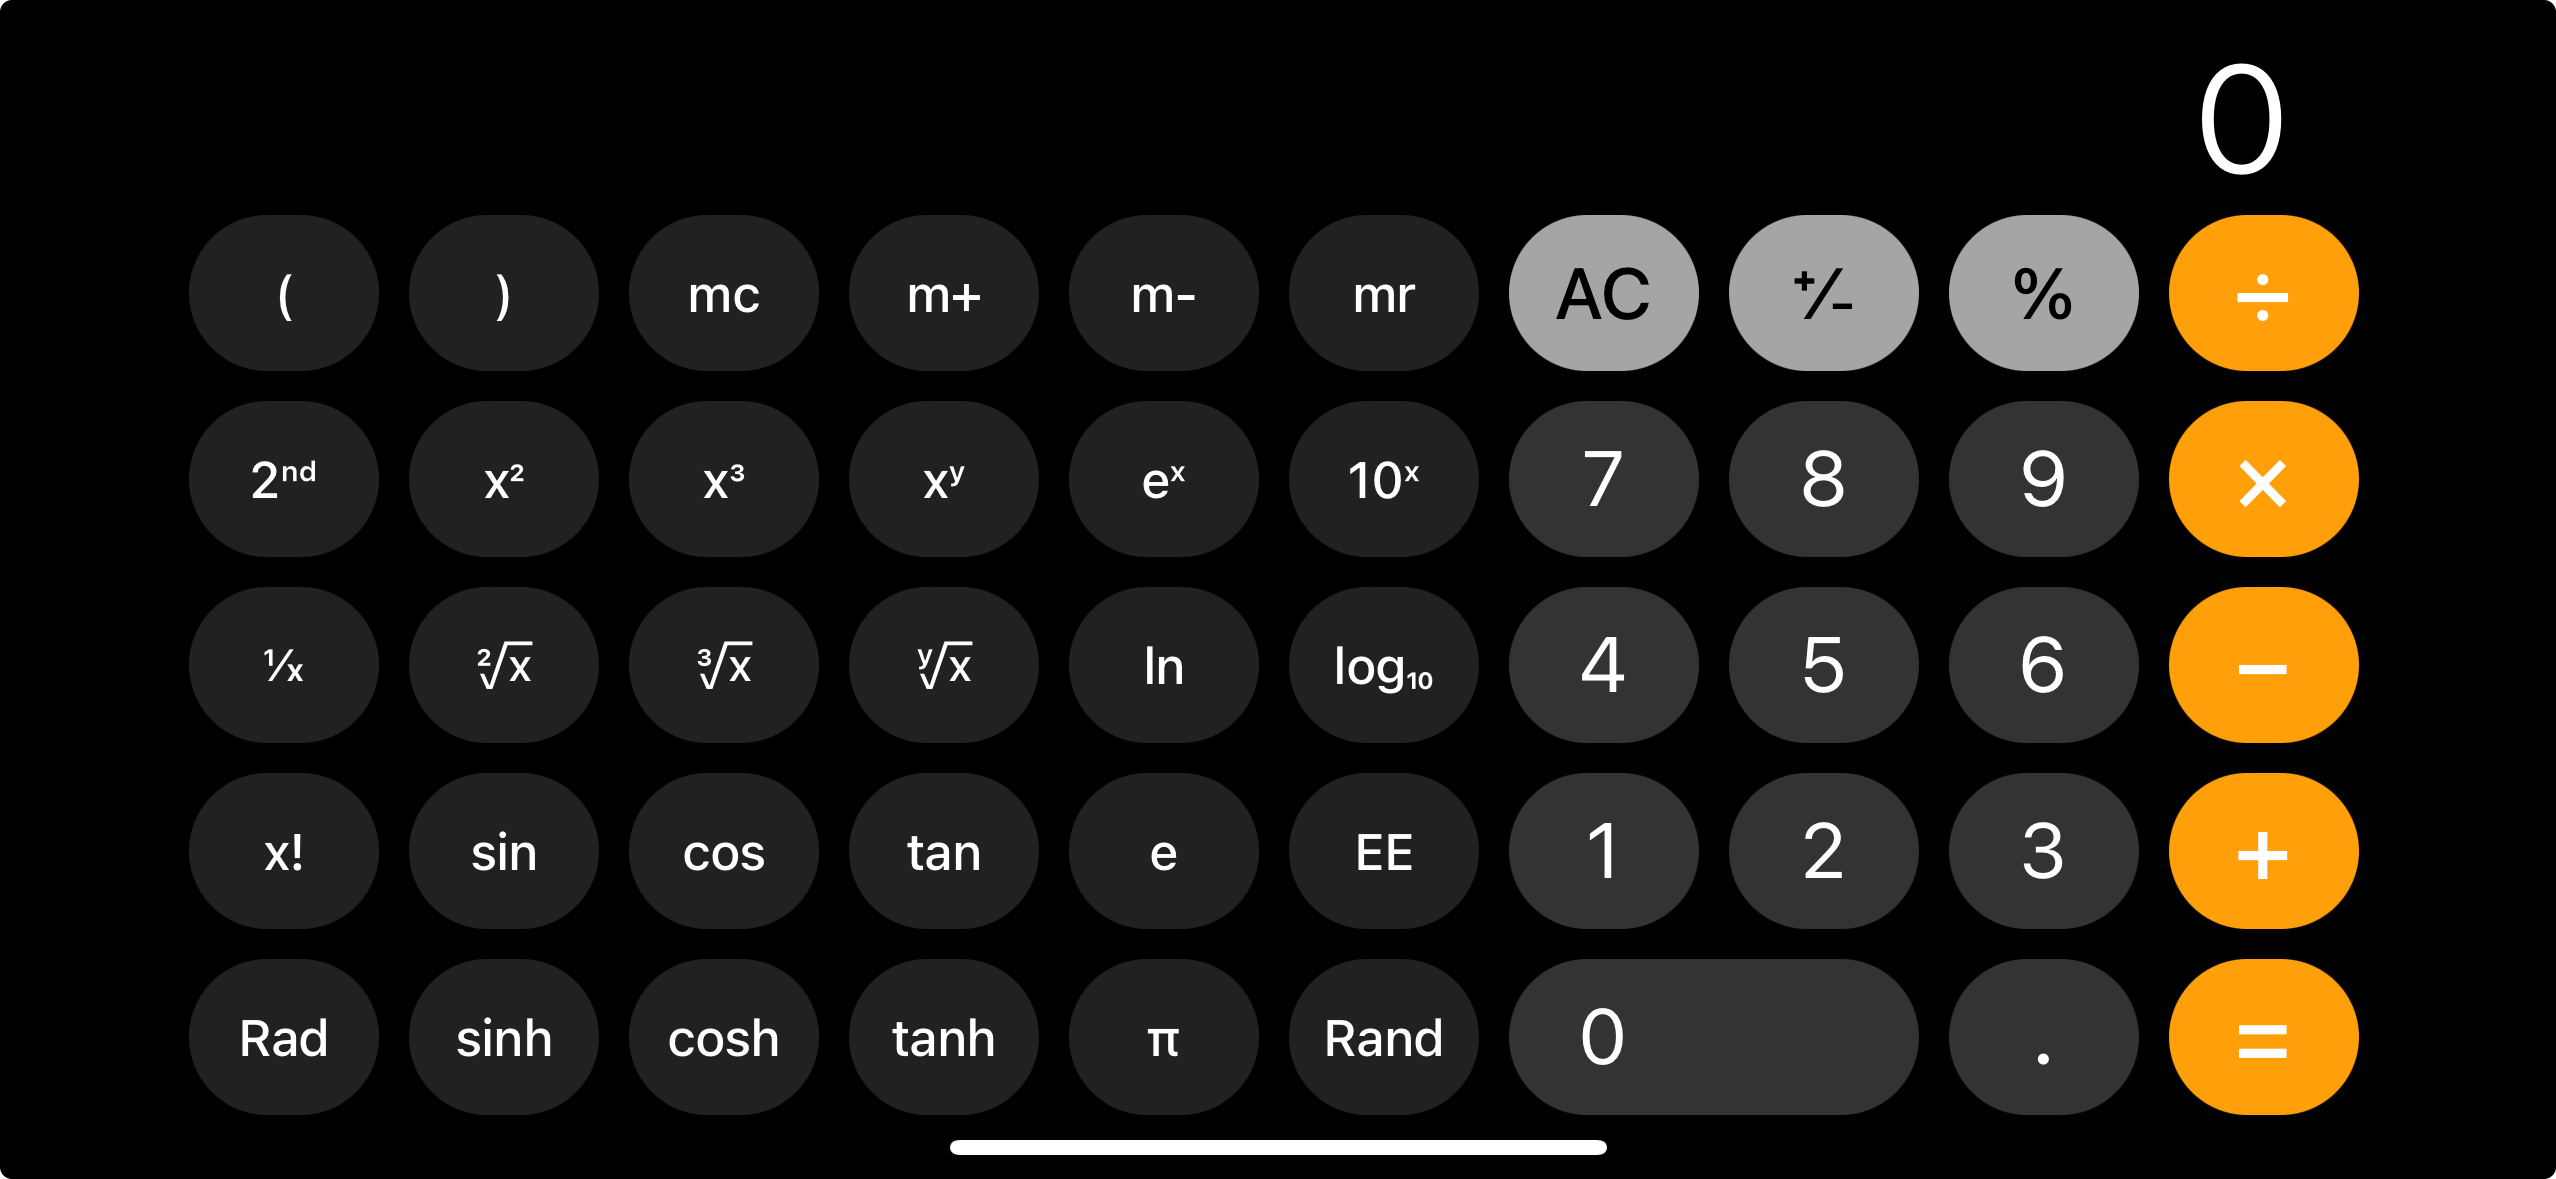
\includegraphics[scale=0.05]{images/iPhoneTR.JPEG}
	\end{minipage}\vspace{5pt}\\
	\begin{aufgabe}
	I	st es möglich die beiden folgenden Logarithmen mit dem Handy-Taschenrechner zu berechnen?
		\begin{enumcols}[2]
			\item $\log{10}{1000}=$
			\item $\log{3}{5}=$
		\end{enumcols}
		\karos{2.5}
	\end{aufgabe}
	Wir sehen also die Basis, die auf diesen Tasten hinterlegt ist, ist entscheidend, um das korrekte Resultat zu erhalten. Aus diesem Grund haben wir zu Beginn die drei speziellen Logarithmen hervorgehoben. Gibt es eine Möglichkeit trotz den Einschränkungen auf dem Handy-Taschenrechner einen beliebigen Logarithmus zu berechnen?  Betrachten wir dazu ein Beispiel.
	\begin{beispiel}
		Wir wollen den folgenden Logarithmus berechnen:
		\begin{gridspace}{8.5}
			\hspace{4pt}$\ds \log{3}{5}=$
		\end{gridspace}
	\end{beispiel}
	\begin{satz}[Basiswechselsatz]\label{satz:Basiswechsel}
		Der Logarithmus einer Zahl zu einer \flqq unbequemen\frqq\:Basis $u$ kann mit der folgenden Gleichung umgewandelt werden: \[\log{u}{b}=\frac{\log{c}{b}}{\log{c}{u}}\]
		\textbf{Wichtig: }$c$ kann frei gewählt werden!
	\end{satz}
	\begin{aufgabe}
		\begin{enumerate}
			\item Berechne die folgenden Logarithmen ausschliesslich mit dem Handy-Taschenrechner.
			\begin{enumcols}[3]
				\item $\log{2}{10}\approx$\:\rule{1.7cm}{1pt}
				\item $\log{}{50}\approx$\:\rule{1.7cm}{1pt}
				\item $\log{15}{11}\approx$\:\rule{1.7cm}{1pt}
				\item $\log{5}{17}\approx$\:\rule{1.7cm}{1pt}
				\item $\log{3}{29}\approx$\:\rule{1.7cm}{1pt}
				\item $\log{2}{-0.1}\approx$\:\rule{1.7cm}{1pt}
				\item $\log{8}{0.8}\approx$\:\rule{1.7cm}{1pt}
				\item $\log{\e}{1000}\approx$\:\rule{1.7cm}{1pt}
				\item $\log{5}{\frac{1}{3}}\approx$\:\rule{1.7cm}{1pt}
			\end{enumcols}
			\item Schreibe die folgenden Logarithmen zur Basis $10$ um.
			\begin{enumcols}[4]
				\item $\log{100}{1000}$
				\item $\log{0.1}{10}$
				\item $\log{2}{5}$
				\item $\log{3}{\abs{x}^{10}}$
			\end{enumcols}
			\item Vereinfache zu einen einzigen Logarithmus.
			\begin{enumcols}[4]
				\item $\ds\frac{\log{10}{2}}{\log{10}{\e}}$
				\item $\ds\frac{\ln{7}}{\ln{10}}$
				\item $\ds\frac{\ln{64}}{\ln{\sqrt{3}}}$
				\item $\ds\frac{\ln{125}}{\ln{8}}$
			\end{enumcols}
			\item Vereinfache die folgenden Ausdrücke, in dem du die Logarithmen zu einer geeigneten Basis wechselst.
			\begin{enumcols}[2]
				\item $\ds\log{3}{4}\*\log{4}{5}\*\log{5}{9}$
				\item $\ds\frac{\log{3}{13}\*\log{5}{17}}{\log{2}{289}\*\log{5}{169}}$
				\item $\ds\frac{\log{3}{125}\*\log{2}{\sqrt[3]{3}}}{\log{8}{5}}$
			\end{enumcols}
			\item Löse die folgende Logarithmusgleichungen nach $x$ auf.
			\begin{enumcols}[2]
				\item $\log{4}{9}=\log{2}{x}$
				\item $\log{3}{16}=\log{x}{256}$
				\item $\log{4}{\log{2}{x}-1}=\log{16}{9}$
			\end{enumcols}
		\end{enumerate}
	\end{aufgabe}
	Mit Hilfe des Basiswechselsatz sind wir also in der Lage, auch ohne leistungsfähigen Taschenrechner einen Logarithmus mit komplizierter Basis zu vereinfachen. Insbesondere können wir so auch die Lösung einer Exponentialgleichung der Form $a^x=b$ mit Hilfe des Basiswechselsatz approximieren. Denn es gilt:
	\[x=\log{a}{b}=\frac{\log{c}{b}}{\log{c}{a}}=\frac{\ln{b}}{\ln{a}}\]\newpage
	\begin{aufgabe}
		Löse die folgenden Exponentialgleichungen auf 4 wesentliche Stellen.
		\begin{enumcols}[3]
			\item $2^x=11$
			\item $3^x=0.052$
			\item $0.8^x=0.005$
			\item $\e^x=\pi$
			\item $\e^{-x}=100$
			\item $\e^{2x-5}=3$
			\item $10^x=1968$
			\item $8\*3^{-x}=5$
			\item $10^6\*0.9^x=\e$
			\item $5^{x-1}+6^x=6^{x+1}-5^x$
			\item $2^{4x}+2^{4x+5}=99$
			\item $5^{3x+1}-5^{3x-1}=48$
			\item $3\*4^x+5=6\*4^x-19$
			\item $9^{x+\frac{1}{2}}-9^x=9^{x-\frac{1}{2}}+135$
		\end{enumcols}
	\end{aufgabe}

\subsection{Vergleich von Zahlen}
	In der folgenden Aufgabe sind zwei Potenzen gegeben, die für unseren einfachen Handy-Taschenrechner leider nicht möglich sind zu berechnen. Also können wir auch nicht einen direkten Vergleich anstellen. Notiere dir hier deinen Tipp.
	\begin{aufgabe}
		Welche Zahl ist grösser? \[2^{2000}\qquad\text{ oder }\qquad 3^{630}\]
	\end{aufgabe}
	Wie kann ich nun rechnerisch überprüfen, welcher dieser Potenzen grösser ist?\vspace{5pt}\newline\karos{4}
	\begin{aufgabe}
		\begin{enumerate}[label=\alph*)]
			\item Welche der folgenden Zahlen ist grösser? Begründe deine Antwort. \[0.9^{3000}\qquad\text{ oder }\qquad 0.8^{1500}\]
			\item Wie viele Ziffern besitzt die im Zehnersystem geschriebene ausgerechnete Potenz?
			\begin{itemize}[label=\ ]\begin{multicols}{4}
					\item $837^{837}$ \item $2^{2000}$ \item $\left(8^7\right)^6$ \item $6^{\left(7^8\right)}$
			\end{multicols}\end{itemize}
			\footnotesize\textit{Tipp: Denke an die wissenschaftliche Schreibweise.}\normalsize
			\item Gib für die obigen 4 Potenzen die erste Ziffer des ausgeschriebenen Wertes an.
		\end{enumerate}
	\end{aufgabe}


\subsection*{Richterskala}
\subsection*{pH-Werte}
\subsection*{C-14 Methode}
\subsection*{Stetige Rendite}
\subsection*{Logarithmus im Tennis}
\subsection*{Widerspenstige Zähmung}
\endgroup
\end{document}